% Version 1

\documentclass[10pt]{llncs}

\usepackage{ucs}
\usepackage[utf8]{inputenc}
\usepackage{amsmath}
\usepackage{amsfonts}

\let\proof\relax
\let\endproof\relax

\usepackage{mathtools}
\usepackage{amsthm}
\usepackage{stmaryrd}
\usepackage{tikz}
\usetikzlibrary{calc}
\usepackage[noend]{algpseudocode}
\usepackage{algorithm}
\usepackage{xcolor}
\usepackage{graphicx}
\usepackage{multirow}
\usepackage{changepage}
\usepackage{todonotes}
\usepackage{comment}
\usepackage{blkarray}
\usepackage[symbol]{footmisc}
\usepackage[tableposition=top]{caption}
\usepackage[left=2.5cm,right=2.5cm]{geometry}

\usepackage{placeins}

\let\Oldsection\section
\renewcommand{\section}{\FloatBarrier\Oldsection}

\let\Oldsubsection\subsection
\renewcommand{\subsection}{\FloatBarrier\Oldsubsection}

\let\Oldsubsubsection\subsubsection
\renewcommand{\subsubsection}{\FloatBarrier\Oldsubsubsection}


\newcommand{\QQIF}[1] {\State \textbf{if} (#1)}
\newcommand{\QQRETURN} {\textbf{return} }

\title{The Maximum Matrix Contraction problem : Appendix\\ WORK IN PROGRESS}
\author{
	Dimitri Watel\inst{1,2}
\and
	Pierre-Louis Poirion\inst{1,3}}
\institute{
 CEDRIC-CNAM, 292 rue du faubourg Saint Martin, 75003, Paris, FRANCE
\and
 ENSIIE, 1 Square de la résistance, Evry, FRANCE
  \email{dimitri.watel@ensiie.fr, }
\and
ENSTA Paristech, 828 boulevard des Maréchaux, 91120, Palaieau, FRANCE
\email{pierre-louis.poirion@ensta-paristech.fr}
}

\usepackage{caption}
\captionsetup[table]{aboveskip=5pt, }

\setcounter{secnumdepth}{3}


\newcommand{\gridsize}{0.5}
\newcommand{\prgrid}[3]{\draw[step=\gridsize,gray,very thin] (#1) grid (\gridsize*#3,\gridsize*#2);}
\newcommand{\prtline}[3]{}%\draw[] ($(#1)+(0,\gridsize*#2)$) -- ($(#1)+(\gridsize*#3,\gridsize*#2)$);}
\newcommand{\prtcolumn}[3]{}%\draw[] ($(#1)+(\gridsize*#2,0)$) -- ($(#1)+(\gridsize*#2,\gridsize*#3)$);}
\newcommand{\prvtline}[3]{\draw[very thick] ($(#1)+(0,\gridsize*#2)$) -- ($(#1)+(\gridsize*#3,\gridsize*#2)$);}
\newcommand{\prvtcolumn}[3]{\draw[very thick] ($(#1)+(\gridsize*#2,0)$) -- ($(#1)+(\gridsize*#2,\gridsize*#3)$);}
\newcommand{\prvtdline}[3]{\draw[very thick,dotted] ($(#1)+(0,\gridsize*#2)$) -- ($(#1)+(\gridsize*#3,\gridsize*#2)$);}
\newcommand{\prvtdcolumn}[3]{\draw[very thick,dotted] ($(#1)+(\gridsize*#2,0)$) -- ($(#1)+(\gridsize*#2,\gridsize*#3)$);}

\newcommand{\prvtdlinec}[4]{\draw[very thick,dotted,color=#4] ($(#1)+(0,\gridsize*#2)$) -- ($(#1)+(\gridsize*#3,\gridsize*#2)$);}
\newcommand{\prvtdcolumnc}[4]{\draw[very thick,dotted,color=#4] ($(#1)+(\gridsize*#2,0)$) -- ($(#1)+(\gridsize*#2,\gridsize*#3)$);}

\newcommand{\prone}[3]{\draw ($(#1)+(#3*\gridsize-0.5*\gridsize,#2*\gridsize-0.5*\gridsize)$) node {$1$};}
\newcommand{\pronec}[4]{\draw[color=#4] ($(#1)+(#3*\gridsize-0.5*\gridsize,#2*\gridsize-0.5*\gridsize)$) node {$1$};}


\renewenvironment{comment}{\begingroup\sffamily\color{red} \itshape}{\endgroup}
\newcommand{\transpose}[1]{\ensuremath{#1^{\scriptscriptstyle T}}}

\renewcommand{\thefootnote}{\fnsymbol{footnote}}

\begin{document}




\theoremstyle{plain}
\newtheorem{corol}{Corollary}

\maketitle

\begin{abstract}
In this paper, we introduce the {\it Maximum Matrix Contraction problem}, where we aim to contract as much as possible a binary matrix in order to maximize its density.  We study the complexity and the polynomial approximability of the problem. Especially, we prove this problem to be NP-Complete and that every algorithm solving this problem is at most a $2\sqrt{n}$-approximation algorithm where $n$ is the number of ones in the matrix. We then focus on efficient algorithms to solve the problem: an integer linear program and three heuristics.\\
\textit{Keywords:} Complexity, Approximation algorithm, Linear Programming
\end{abstract}

This document contains the appendix of a paper accepted at the conference ISCO 2016, this appendix could not be added to the camera-ready version due to lack of space. This document is presently incomplete, some explanations are missing, but it should be completed soon.

\appendix

\section{An instance with an $O(\sqrt{n})$ gap between the worst and the best solution.}

\label{apx:badinstance}


Theorem~\ref{theo:sqrtnapprox} of Section~\ref{sect:approx} proves a default $2\sqrt{n}$ upper bound of the approximation ratio for every algorithm returning a maximal solution.

We give, in this appendix, in Figure~\ref{fig:badinstance}, an instance in which the ratio between an optimal density and the lowest density of a maximal solution is at least $4\sqrt{n}$.

\begin{figure}
    \centering

    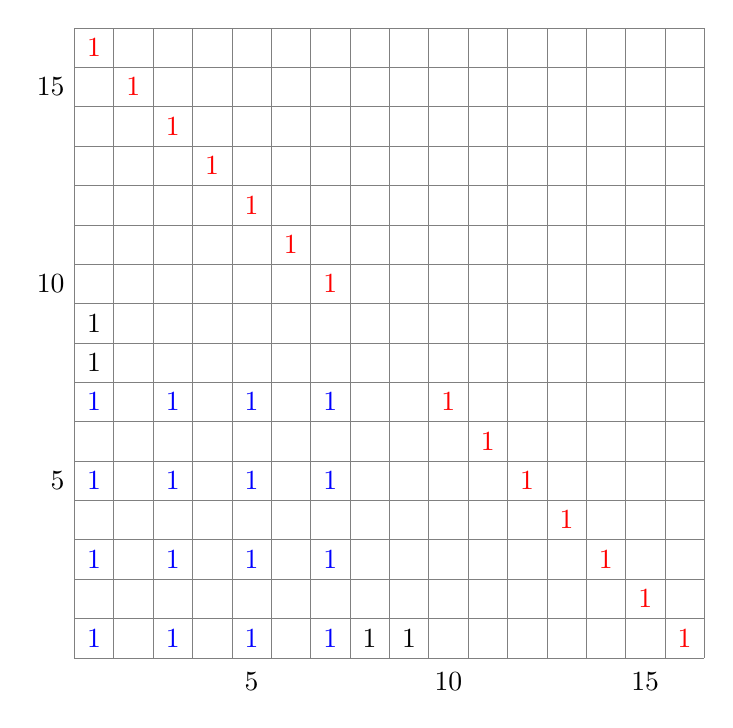
\begin{tikzpicture}
        \coordinate (O) at (0,0);
        \prgrid{O}{16}{16}

\definecolor{tempcolor}{rgb}{0.0,0.0,1.0}
        \pronec{O}{1}{1}{tempcolor};
\definecolor{tempcolor}{rgb}{0.0,0.0,1.0}
        \pronec{O}{1}{3}{tempcolor};
\definecolor{tempcolor}{rgb}{0.0,0.0,1.0}
        \pronec{O}{1}{5}{tempcolor};
\definecolor{tempcolor}{rgb}{0.0,0.0,1.0}
        \pronec{O}{1}{7}{tempcolor};
\definecolor{tempcolor}{rgb}{0.0,0.0,0.0}
        \pronec{O}{1}{8}{tempcolor};
\definecolor{tempcolor}{rgb}{0.0,0.0,0.0}
        \pronec{O}{1}{9}{tempcolor};
\definecolor{tempcolor}{rgb}{1.0,0.0,0.0}
        \pronec{O}{1}{16}{tempcolor};

\definecolor{tempcolor}{rgb}{1.0,0.0,0.0}
        \pronec{O}{2}{15}{tempcolor};

\definecolor{tempcolor}{rgb}{0.0,0.0,1.0}
        \pronec{O}{3}{1}{tempcolor};
\definecolor{tempcolor}{rgb}{0.0,0.0,1.0}
        \pronec{O}{3}{3}{tempcolor};
\definecolor{tempcolor}{rgb}{0.0,0.0,1.0}
        \pronec{O}{3}{5}{tempcolor};
\definecolor{tempcolor}{rgb}{0.0,0.0,1.0}
        \pronec{O}{3}{7}{tempcolor};
\definecolor{tempcolor}{rgb}{1.0,0.0,0.0}
        \pronec{O}{3}{14}{tempcolor};

\definecolor{tempcolor}{rgb}{1.0,0.0,0.0}
        \pronec{O}{4}{13}{tempcolor};

\definecolor{tempcolor}{rgb}{0.0,0.0,1.0}
        \pronec{O}{5}{1}{tempcolor};
\definecolor{tempcolor}{rgb}{0.0,0.0,1.0}
        \pronec{O}{5}{3}{tempcolor};
\definecolor{tempcolor}{rgb}{0.0,0.0,1.0}
        \pronec{O}{5}{5}{tempcolor};
\definecolor{tempcolor}{rgb}{0.0,0.0,1.0}
        \pronec{O}{5}{7}{tempcolor};
\definecolor{tempcolor}{rgb}{1.0,0.0,0.0}
        \pronec{O}{5}{12}{tempcolor};

\definecolor{tempcolor}{rgb}{1.0,0.0,0.0}
        \pronec{O}{6}{11}{tempcolor};

\definecolor{tempcolor}{rgb}{0.0,0.0,1.0}
        \pronec{O}{7}{1}{tempcolor};
\definecolor{tempcolor}{rgb}{0.0,0.0,1.0}
        \pronec{O}{7}{3}{tempcolor};
\definecolor{tempcolor}{rgb}{0.0,0.0,1.0}
        \pronec{O}{7}{5}{tempcolor};
\definecolor{tempcolor}{rgb}{0.0,0.0,1.0}
        \pronec{O}{7}{7}{tempcolor};
\definecolor{tempcolor}{rgb}{1.0,0.0,0.0}
        \pronec{O}{7}{10}{tempcolor};

\definecolor{tempcolor}{rgb}{0.0,0.0,0.0}
        \pronec{O}{8}{1}{tempcolor};

\definecolor{tempcolor}{rgb}{0.0,0.0,0.0}
        \pronec{O}{9}{1}{tempcolor};

\definecolor{tempcolor}{rgb}{1.0,0.0,0.0}
        \pronec{O}{10}{7}{tempcolor};

\definecolor{tempcolor}{rgb}{1.0,0.0,0.0}
        \pronec{O}{11}{6}{tempcolor};

\definecolor{tempcolor}{rgb}{1.0,0.0,0.0}
        \pronec{O}{12}{5}{tempcolor};

\definecolor{tempcolor}{rgb}{1.0,0.0,0.0}
        \pronec{O}{13}{4}{tempcolor};

\definecolor{tempcolor}{rgb}{1.0,0.0,0.0}
        \pronec{O}{14}{3}{tempcolor};

\definecolor{tempcolor}{rgb}{1.0,0.0,0.0}
        \pronec{O}{15}{2}{tempcolor};

\definecolor{tempcolor}{rgb}{1.0,0.0,0.0}
        \pronec{O}{16}{1}{tempcolor};

\draw ($(O)+(0,2.25)$) node[anchor=east] {$5$};
\draw ($(O)+(0,4.75)$) node[anchor=east] {$10$};
\draw ($(O)+(0,7.25)$) node[anchor=east] {$15$};
\draw ($(O)+(2.25,-0.3)$) node {$5$};
\draw ($(O)+(4.75,-0.3)$) node {$10$};
\draw ($(O)+(7.25,-0.3)$) node {$15$};

    \end{tikzpicture}
    \caption{An example of grid in which the gap between an optimal solution and the worst maximal solution is $O(\sqrt{n})$.}
    \label{fig:badExample}
\end{figure}


We highly believe this instance is the worst case that can happen and that the density of a maximal solution is always higher than $4\sqrt{n}$. The result of Theorem~\ref{theo:sqrtnapprox} may then possibly be updated to the following conjecture. 

\begin{conjecture}
	An algorithm returning any maximal solution of an instance of MMC is a $\sqrt{n}$-approximation.
\end{conjecture}

\end{document}